\documentclass[12pt,a4paper, twocolumn]{article}
\usepackage[utf8]{inputenc}
\usepackage[english]{babel}
\usepackage{amsmath}
\usepackage{amsfonts}
\usepackage{amssymb}
\usepackage{graphicx}
%\usepackage[left=2cm,right=2cm,top=2cm,bottom=2cm]{geometry}
\usepackage{lipsum}
\usepackage{multicol}
\usepackage{float}

\floatstyle{boxed}
\restylefloat{figure}
\setlength\columnsep{15pt}

\author{Baptiste \textsc{Rouger} \and Fanny \textsc{Roussel}}
\title{Report :\\Experimental Methods}
\date{February 20$^{\text{th}}$, 2017} 

\begin{document}
\maketitle

\begin{abstract}
Cryptobiosis is the phenomenon that consists in slowing down the metabolism of an organism in order to extend its life. This phenomenon can be studied in small multicellular organisms that are able to do it : the tardigrads. We studied the time required to set up this state in \textit{Hypsibius dujardini}. We have been able to show that, with an increasing concentration of NaCl, the average time required to observe half of the tardigrads in the cryptobiosis state was decreasing accordingly. Furthermore, we show that the higher the stress, the harder it is to go in cryptobiosis. Study this mecanism could lead to better the cryogenesis currently used and preserve both model organisms like bacterias and humans from aging.
\end{abstract}

%\begin{multicols}{2}

\section{Introduction}
Tardigrads (species : \textit{Hypsibius dujardini}) are small animals known in the literature as capable of resisting extreme conditions. They have the ability to enter into cryptobiosis in order to protect themselves from temperature variations (cryobiosis), dehydration (anhydrobiosis), lack of oxygen (anoxybiosis) or high salt concentrations (osmobiosis). Confronted to a stress, tardigrades are entering a reversible suspended  and contracted metabolic state, losing more than 95\% of their water and secreting trehalose, a sugar aimed at protecting their cells. Once back in a friendly environment, tardigrades can get out of the tun conformation, generally after a few hours, and behave normally again.\\
The aim of our project was to observe tardigrades confronted to different intensities of a specific stress, and their response over time in terms of tun formation or death. We decided to put our cultured tardigrades in different concentrations of NaCl – one of the stress they are known to be able to resist to – and observe the evolution of the population : we knew that if tardigrades are confronted to a stress, they need to protect themselves. If not, they die. Our protocol was thus to inject a certain quantity of NaCl solution in the tardigrades’ environment and track the population behaviour every two minutes until no tardigrade is moving in the observed sample anymore : they would either be in tuns or dead.\\
 
If these animals are known to survive almost any stress as tuns, they are indeed quite sensitive while out of this conformation :


\section{Methods}
In order to test the effect of the concentration of salt on the time required to get in tun conformation by the tardigrads depending on the concentration of salt, we used homemade multiwell plates (c.f. \textsc{Section} DIY) in which we placed 5 $\mu$L of a solution of cultured tardigrads, and 5 $\mu$L of a solution of NaCl at twice the concentration we wanted to obtain. We then set our slides under the microscope and count the number of living tardigrads we observe in the well to ensure a representative number. We then count every two minutes the number of living, dead, and tun tardigrads (\textsc{Figure}~\ref{dead-tun}). We make kinetics on a maximal length of 50 minutes, with an other measure at 60 minutes. Though, if we observed no living tardigrads for 6 consecutive minutes, we stopped the measure. Moreover, at 30 minutes, we added 5 $\mu$L of water in order to compensate the water lost by evaporation.\\
We experimented on the tardigrads with different concentrations of NaCl such as $0.000$M, $0.050$M, $0.065$M, $0.080$M and $0.100$M.\\
We developped several index to represent the number of living, tun, and dead tardigrads. The first one is the proportion of one category of tardigrad over the whole population $\frac{\text{Active, Tun or Dead}}{\text{Whole population}}$. The second index represent the proportion of tun tardigrads over the living population $\frac{\text{Tun}}{\text{Tun}+ \text{Active}}$. With these, we can represent the kinetics of the number of tardigrads that are active, in tun, or dead.\\
The last index we created is the half-time to conformation change ($tcc_{1/2}$), which represents the time at which half of the living (active + tun) tardigrads are in the tun conformation. With it, we can have a representation of how fast do the tardigrads change of conformation, and go in osmobiosis.

\begin{figure}
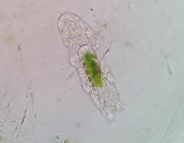
\includegraphics[width=0.49\linewidth]{dead.png}
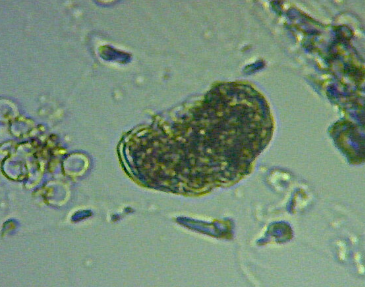
\includegraphics[width=0.49\linewidth]{tun.png}
The conformation of the tardigrads presented in these pictures are our base to determine them. The first picture represents a dead tardigrad (relaxed conformation, no movement), the second pictures shows a tun tardigrad (ball shape, no movement). We consider the tardigrads as active if they are moving.
\label{dead-tun}
\caption{The different conformations of the tardigrads}
\end{figure}


\section{Results}
\lipsum[20]
\section{Discussion}
\lipsum[20]

\newpage
\section*{Problems raised during the experiments}
\lipsum[20]

\section*{DIY}
\lipsum[20]






%\end{multicols}
\end{document}
